
%%%%%%%%%%%%%%%%%%%%%%%%%%%%%%%%%%%%%%%%%%%%%%%%%%%%%%%%%%%%%%5
%% Thesis Author: Joshua Daly - b00056835@student.itb.ie
%% ITB Author: Markus Hofmann - markus.hofmann@itb.ie
%% Adapted from Dalhousie University
%%%%%%%%%%%%%%%%%%%%%%%%%%%%%%%%%%%%%%%%%%%%%%%%%%%%%%%%%%%%%%%5

\documentclass[12pt]{report}

\usepackage{amsfonts}
\usepackage{amssymb,amsmath}
\usepackage{amsthm}
\usepackage{newlfont}
\usepackage{graphicx}
\usepackage{tabularx}
\usepackage{longtable}
\usepackage{lscape}
\usepackage{latexsym}
\usepackage{geometry}
\usepackage{fancyhdr}
\usepackage{xthesis}
\usepackage{xtocinc} 
\usepackage{subfigure}
\usepackage{times}
\usepackage[hidelinks]{hyperref}
%\usepackage{color}
\usepackage{listings}
\usepackage{hyperref}

%\definecolor{dkgreen}{rgb}{0,0.6,0}
%\definecolor{gray}{rgb}{0.5,0.5,0.5}
%\definecolor{mauve}{rgb}{0.58,0,0.82}

\lstset{frame=tb,
  language=Python,
  aboveskip=3mm,
  belowskip=3mm,
  showstringspaces=false,
  columns=flexible,
  basicstyle={\small\ttfamily},
  numbers=none,
  %numberstyle=\tiny\color{gray},
  %keywordstyle=\color{blue},
  %commentstyle=\color{dkgreen},
  %stringstyle=\color{mauve},
  breaklines=true,
  breakatwhitespace=true,
  tabsize=3
}

\bibliographystyle{ieeetr}

% Line spacing -----------------------------------------------------------
\newlength{\defbaselineskip}
\setlength{\defbaselineskip}{\baselineskip}
\newcommand{\setlinespacing}[1]%
           {\setlength{\baselineskip}{#1 \defbaselineskip}}
\newcommand{\doublespacing}{\setlength{\baselineskip}%
                           {2.0 \defbaselineskip}}
\newcommand{\singlespacing}{\setlength{\baselineskip}{\defbaselineskip}}
% ------------------------------------------------------------------------
\makeatletter
\renewcommand\appendix{%
 \par
 \setcounter{chapter}{0}%
 \setcounter{section}{0}%
 \setcounter{subsection}{0}%
 \gdef\thesection{\@Alph\c@section}
 \gdef\@sect##1##2##3##4##5##6[##7]##8{%
  \refstepcounter{##1}%
  \protected@edef\@svsec{\@seccntformat{##1}\relax}%
  \begingroup
    \hspace{-\parindent}##6\appendixname~ {%
    \@hangfrom{\hskip ##3 \relax\@svsec}\par%
    \hspace{-\parindent}\interlinepenalty \@M ##8 \@@par}%
  \endgroup
  \csname ##1mark\endcsname{##7}%
  \addcontentsline{toc}{##1}{\protect\numberline{\csname the##1\endcsname}##7}%
  \@xsect{##5}%
 }%
}%
\makeatother
%%% ----------------------------------------------------------------------

\begin{document}

\setlinespacing{1.5}

\title{An Analysis of the Field D* Algorithm for Path Planning in the Return and Delivery Journey of Ground Based Courier Robots}

\author{Joshua Daly}

\university{Institute of Technology Blanchardstown}

\dept{School of Informatics and Engineering}

\address{Dublin, Ireland}

\supervisor{Mr. Arnold Hensman}

\submitdate{\today}

\degree{B.Sc. (Honours) in Computing}

%\dedicate{To my wife\\
% \begin{Huge}{\textbf{Glenda}}\end{Huge}}

\beforepreface

{ 
\typeout{Abbreviations}
% Thesis Abbreviation ------------------------------------------------------

\prefacesection{Abbreviations}


%%%%%%%%%%%%%%%%%%%%%%%%%%%%%%%%%%%%%%%%%%%%%%%%%%%%%%%%%%%%%%%%%%%%%%%%%%%%%%%%
% Create a list of all abbreviations that you've used throughout your thesis.  %
% Order the abbreviations in alphabetical order                                %
%%%%%%%%%%%%%%%%%%%%%%%%%%%%%%%%%%%%%%%%%%%%%%%%%%%%%%%%%%%%%%%%%%%%%%%%%%%%%%%%

\begin{longtable}{p{90pt}l}
\hline DARPA		 & Defence Advanced Research Project Agency \\ 
\hline SLAM      & Simultaneous Localisation and Mapping \\
\hline
\end{longtable}






% ----------------------------------------------------------------------
 %write your list of abbreviations in a file called abbreviations.tex
}

%{ 
%\typeout{Glossary}
%\include{glossary}
%}

% ------------------------------------------------------------------------
\afterpreface
%\def\baselinestretch{1}
% ------------------------------------------------------------------------

\pagestyle{fancy}
\setcounter{page}{1}

%\chapter{Introduction}

%-------------------------------------------------------------------------------------------------------

\section{Background}

\noindent
Provide a context to the reader, talk about the project, where the idea came from (extension of 3rd Project), some examples of courier robots today. Summary of the big industry players like Google and Amazon. Why is the project unique. Most of this can be taken from the background provided with the project proposal and literature review submissions for Research Skills.\\

\noindent
The ability to select a path to a destination, negotiate obstacles, and anticipate the movement of other people is something that you probably take for granted. To a human these skills are a part of everyday life and do not at first appear to be particularly special, until you try to replicate them. Programming a machine to deal with rush hour traffic or road closures is surprisingly difficult but that has not stop us from trying \cite{MIT}.\\

%-------------------------------------------------------------------------------------------------------

\section{Motivation}

\noindent
This section is a combination of the \textit{Justifications and Benefits} and \textit{Feasibility} sections from the project proposal and should state the following:

\begin{itemize}
\item Primary reason for undertaking this project, probably academic.
\item Any potential benefits to society and ITB developing this technology has.
\item The fact it evolved from a 3rd project and reuses existing equipment.
\item Back all this up with sound evidence that suggests that this project has an achievable goal.
\end{itemize} 

%-------------------------------------------------------------------------------------------------------

\section{Scope Definition}

\noindent
What is the actual scope of this project? Defining what to exclude is just as important as what is included so state both of these here in bullet points:\\

\noindent
The scope of this project \textbf{includes}:
\begin{itemize}
\item Path Planning: calculating the shortest and safest path to the delivery point.

\item State everything else...
\end{itemize}

\noindent
The following are \textbf{outside} the scope of this project:
\begin{itemize}
\item Collection: purely automated collection using beacons or computer vision. Goods will be manually handled by a human operator.

\item State everything else...
\end{itemize}

%-------------------------------------------------------------------------------------------------------

\section{Research Question(s)}

\noindent
State the primary research question of this project on its own line possibly in bold or italics. Then follow it with other sub research questions in bullet points:

\begin{itemize}
\item Where can mobile delivery robots be used outside of research laboratories?

\item State everything else...
\end{itemize}

%-------------------------------------------------------------------------------------------------------

\newpage

\section{Objectives}

\noindent
One line introducing the purpose of these objectives followed by the objectives themselves again in bullet points:

\begin{itemize}
\item To evaluate the effectiveness of path planning techniques in known and partially known environments.

\item State everything else...
\end{itemize}

%-------------------------------------------------------------------------------------------------------



%\chapter{Literature Review}

%-------------------------------------------------------------------------------------------------------

\section{Courier Robots}

\subsection{Field of Application}

\subsection{Social and Economic Impact}

%-------------------------------------------------------------------------------------------------------

\section{Path Planning}

\subsection{Defining the Problem}

\subsection{Representing the World as a Grid}

%-------------------------------------------------------------------------------------------------------

\section{Path Planning Algorithms}

\subsection{Dijkstra's Algorithm}

\subsection{D* Lite}

\subsection{Field D*}

%-------------------------------------------------------------------------------------------------------

\section{Discussion}



%\chapter{System Design}

%-------------------------------------------------------------------------------------------------------

\section{Requirements Specification}

\subsection{Ability to Plan a Path}
\noindent
The primary functional requirement for this system is the ability to plan a path through a complex environment that can then be traversed by a mobile robot. By a complex environment we refer to a 2D representation stored in some form of map that \textit{may} represent a real world environment. The complexity of the environment is determined by the number of obstacles that the planner must successfully avoid. The success of a journey shall be measured based on the length of the planned path as a percentage when compared to other solutions. \\

\noindent
Given a 2D map, start, and goal position, the planner using \textbf{a path planning algorithm must produce a traversable path}. A path will be made up of a series of points expressed in \textit{x} and \textit{y} coordinates, these can then be iteratively processed. In a case where no path to the goal exists due to obstacles the planning process must be capable of gracefully terminating which includes safely bring the robot to a halt and providing appropriate feedback. \\

\noindent
\textbf{Inputs:} 2D map, start position, goal position \\
\textbf{Outputs:} A path of points OR termination feedback

\newpage

\subsection{Robot Mobility}
\noindent
In order to traverse the path produced as outlined in the previous requirement we need a mobile robot. \textbf{A mobile robot is one that is capable of movement in at least one axis} that will result in a change of position. For our purposes we need to be mobile in both the \textit{x} and \textit{y} axis. The robotic platform's drive system therefore will need to be based on a wheeled, tracked, or legged configuration which can provide the ability to travel on a level surface. It is important to note that the planning system places no restrictions on the dimensions of the robot. \\ 

\noindent
However neither does it account for cases where these dimensions make traversing a path impossible due to space restrictions. The system must be able to make an intelligent decision based on the robot's current position and the next point to travel towards. The output from this requirement is an action that brings us closer towards the goal, this may involve rotating to face the next point along with travelling the calculated distance. \\

\noindent
\textbf{Inputs:} current positon, next postion \\
\textbf{Outputs:} travel distance OR travel distance AND rotate

\subsection{Data Gathering}
\noindent
During the execution of the plannning process the system shall generate a constant stream of data, and a requirement
of this project is to capture this information for later analysis. The type of data being produced can tell us a lot
about the operation including the accuracy, run time, and each planners efficiency. These results must be stored in a permanent way. The data attributes that need to be gathered include the planned path, run time, length of the path, and the total number of vertex accesses. \\

\noindent
\textbf{Inputs:} planned path, run time, length of path, total vertex accesses \\
\textbf{Outputs:} time stamped directory containing datasets and plot files

\subsection{Hardware Platform Specification}
\noindent
As the path planning system implemented on the Linux host is designed to be independent from the hardware specifics of the robot it is necessary that all robots communicate with the planner in a predefined way. We will discuss this mechanism under \ref{sec:protocol} from the software side here we will specify a generic robot that implements the interface. \\

\noindent
In order to be compatible with the planner a robot must have software/hardware:

\begin{itemize}
\item Odometers - capable of establishing an $(x, y)$ position in meters and $\theta$ in radians.
\item Communications - a channel for processing text based data to and from the planner.
\item External Sensors - at least one proximity sensor for detecting obstacles in the environment.
\end{itemize}

\noindent
How accurate this hardware needs to be is completely dependent on the application, the planning system can only assume that any data it receives is valid. Any hardware inaccuracies i.e. drift must be dealt with at a lower level, the purpose of this approach is to decouple the planner from a robot's implementation details. This enables the planning system to be tested across a wide variety of platforms without having to account for each individual hardware configuration (Figure \ref{Figure: Hardware Agent Specification.}). It is perfectly possible that the planner and robot hardware control be implemented on the same physical system rather than externally this could be done via IP using the \textit{localhost} address.

\begin{figure}[htbp]

\center 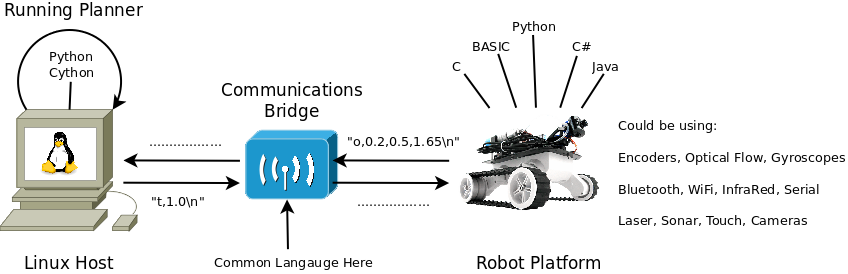
\includegraphics[width=400pt]{illustrations/hardware_agent_specification}\\
\caption{The planner on the Linux host and robot platform communicate via a common communications bridge that they both understand regardless of implementation details.} 
\label{Figure: Hardware Agent Specification.}

\end{figure}

\subsubsection{Motion Model}
\noindent
The planner will impose some restrictions on the motion model that a robot must use to be compatible with the paths it produces. It will be assumed that the robot can perform on the spot rotations, this is necessary as all of the path planning algorithms \textit{may} produce paths that require this kind of motion. In wheeled and tracked vehicles this is typically referred to as \textit{skid steering} \cite{JMD14}, on the spot rotations are achieved by running the drive systems on either side in opposite directions, a tank is good example of this. Legged robots are also capable of performing such turns, however the heading changes can be too extreme for rack-and-pinion based agents i.e. cars and trucks. 

\newpage

%-------------------------------------------------------------------------------------------------------

\section{System Modelling}

\subsection{Overview}
\noindent
The navigation system as a whole is built from four key components that when brought together can be used to evaluate the performance of the selected path planning algorithm. These four components are (Figure \ref{overview}):

\begin{enumerate}
\item \textit{Inputs} - operating map and a valid configuration
\item \textit{System Core} - provides all of the functionality and the interface
\item \textit{Pluggable Algorithms} - deal specifically with producing paths
\item \textit{Physical Output} - actual movement of a mobile robot
\end{enumerate}

\begin{figure}[htbp]

\center 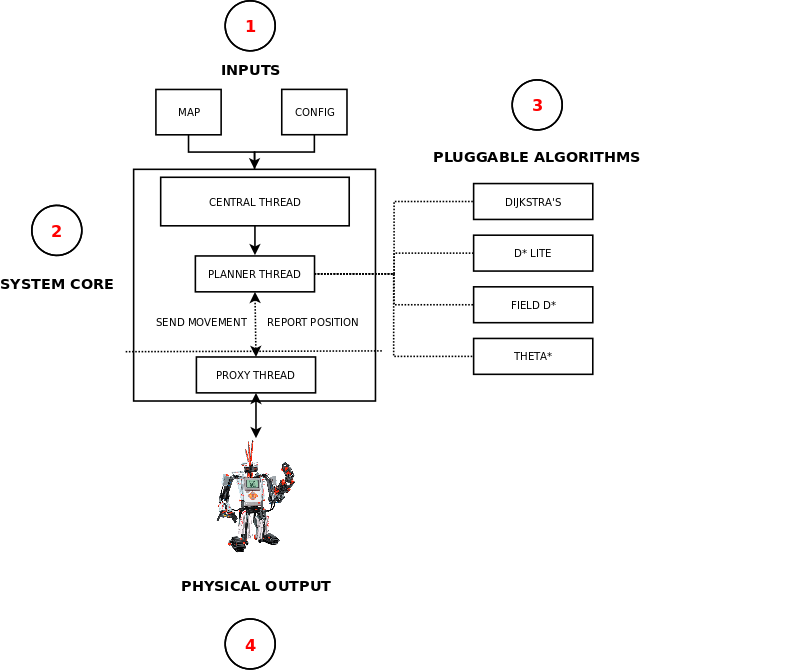
\includegraphics[width=325pt]{illustrations/overview.png}\\
\caption{Individually each component in the system is of limited use but by bringing them together the result is a fully functional path planning system.} 
\label{overview}

\end{figure}

\noindent
In essence the final component \textit{may} not even exist as a physical robot. Instead a computer generated simulation could be used for carrying out large numbers of tests in controlled environments. Each of these components is mutually dependent on the other, we cannot start the system core without both a valid map and configuration, just in the same way without an algorithm there can be no path. This should not be mistaken for \textit{tight coupling}, instead this is a \textit{modular} implementation where each component interacts in an abstract way. When all of these components come together we have a path planning system not just an algorithm.

\subsection{Threaded Architecture}

\noindent
The \textit{BotNav} navigation system contains three separate threads of execution each of which perform a specific task, they are the Central, Proxy, and Planner threads. As threaded programming is notoriously difficult to understand we will cover the architecture here in detail. The task of the three threads can be summarised as follows: 

\begin{itemize}
\item \textbf{Central} - Deals with user input, configuration, initial execution, and pre-emptive termination. 
\item \textbf{Proxy} - Provides a two way communications channel to a physical robot for sending commands and receiving updates.
\item \textbf{Planner} - Interacts with the planning algorithm and produces a string of points that the robot iteratively navigates to.
\end{itemize} 

\subsubsection*{Central Thread}
\noindent
The Central thread deals with user input i.e. the configuration file, based on the parameters in the configuration file it may spawn both the Proxy \textit{and} Planner threads or just the Planner thread. In simulation mode the Central thread will spawn $n$ Planner threads one after another, where $n$ is the total number of traversable cells, as each Planner finishes another begins. In physical mode only one Planner thread is spawned as it is only practical to carry out one journey with a real robot. \textit{BotNav} terminates execution after all of the Central thread's children finish. Below we can see the basic process flow for the Central thread in Figure \ref{central thread}:

\begin{figure}[htbp]

\center 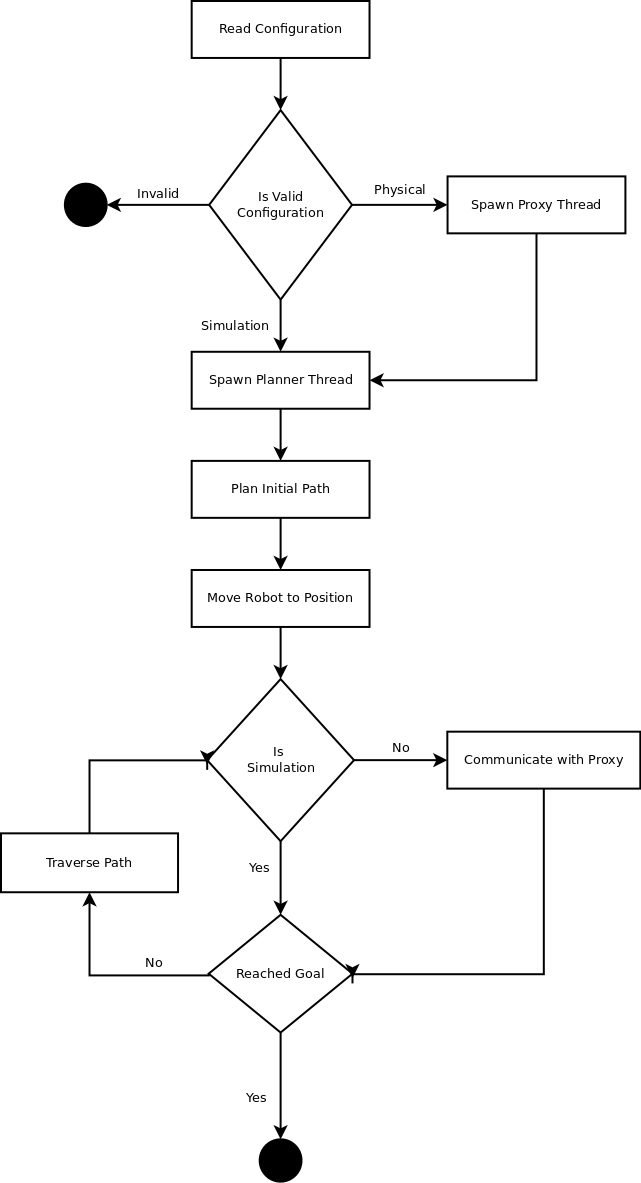
\includegraphics[width=200pt]{illustrations/thread_flow.png}\\
\caption{From reading the configuration file to deciding upon which child threads to spawn, the Central thread plays a very important part in the execution of the system.} 
\label{central thread}

\end{figure}

\subsubsection*{Proxy Thread}
\noindent
Two way communication with a physical robot that implements the communications protocol outlined in \ref{sec:protocol} is provided via the Proxy thread. The Proxy thread's \textit{passive} function is to process the constant stream of odometry data being generated by the robot, this data is then passed onto the system as odometry updates. 

\subsubsection*{Planner Thread}
\noindent
It is in the execution of the Planner Thread where the must crucial work takes place, the Planner brings together a map, robot, proxy, and planning algorithm. All of this is achieved in such a way that it is possible to plug any one of the planning algorithms implemented for this project (GridNav, D* Lite, Field D*, Theta*) into it. \\

\noindent
During a planning cycle the Planner Thread calls upon the planning algorithms \textit{plan} routine which uses a combination of the robot's current position, a goal, and an occupancy grid to produce a path. The actual implementation behind a particular algorithm's planning functionality is hidden from the Planner Thread. If there is a valid path the result of the call to \textit{plan} will be a trail of points which the robot can then iteratively traverse. In the case where no path exists to the goal execution is immediately terminated. \\

\noindent
Once a path has been generated and returned it is processed as follows: \\

\begin{lstlisting}
while we are not within 0.7 cells of the goal in both x and y:
	# Scan the immediate area.
	robot.scan()
	
	# Check for a change in the map.
	if there is a change:
		path = algorithm.plan()
		
	# Pop the next point from the current path.
	if path length is 0:  # Make sure there is a point.
		break

	point = path.pop() # Get the next point.
	robot.go(point.x, point.y)
	
	while robot is travelling:
		# Busy wait.

	calculate x difference to goal
	calculate y difference to goal
\end{lstlisting}

%-------------------------------------------------------------------------------------------------------

\section{Communications Protocol}\label{sec:protocol}
\noindent
This section briefly discusses the communications protocol that a physical hardware robot must implement in order to be compatible with the planning system. The protocol covered here is an extension of the simple communications mechanism from \cite{JMD14} that was used to drive a tele-operated mapping robot. It is based on plain text strings terminated by new line characters (`$\backslash$n') and was designed with simplicity in mind. All commands are synchronous in behaviour and cannot be completed until the appropriate response has been returned. The full specification is available in the Appendices under section \ref{Appendix: Communications Protocol Specification}.

\subsection{Travelling a Predefined Distance}
\noindent
To instruct the robot to travel forward for a straight line distance of 1.3 metres the command is simply: \\

\textit{t,1.3$\backslash$n} \\

\noindent
The `t' character literally stands for \textit{``travel"}, the distance specified as a decimal number comes immediately after the `,' character and can be any \textbf{positive} value, it must be terminated by a newline character. When the robot has completed the command it simply responses with the string: \\

\textit{Travelled$\backslash$n} \\

\noindent
This informs the planner that the robot is no longer in motion and that the next planning step can now be processed. It is possible for a robot's local planner or obstacle avoidance system to abort the action by simply returning this response at any stage in the journey due to unforeseen obstacles. In these cases the robot should return the location of the obstacle(s) in its next scan report.

\subsection{Rotating to a Given Heading}
\noindent
Valid headings run from 0 to 6.27 radians in a circular fashion, they increase from right to left around the circle. To instruct the robot to face a heading of 1.57 radians ($90^{\circ}$) the command is: \\

\textit{r,1.57$\backslash$n} \\

\noindent
There is no explicit return value instead the planner waits until the odometry reports from the robot are within 0.02 radians ($1^{\circ}$) of the requested heading, the robot is then instructed to stop if it has not already done so. The planner uses both the travel and rotation commands in conjunction to navigate to specific points. \\

\noindent
First the robot is commanded to face a given point then the distance between its position and the target are calculated, secondly the robot is sent a travel command containing this information. Using this mechanism the robot is able to navigate complex environments with only the basic knowledge it requires, the rest is done by the planner.

%-------------------------------------------------------------------------------------------------------

\section{Programming Platforms}

\subsection{Linux Architecture}
\noindent
The Linux kernel is to date driving an increasing number of commercial and research robotic platforms all over the world including Google's Self Car Project, Nao, EV3 Lego Mindstorms, and the horde of robots that use ROS \cite{MIT, NAO, EV3, ROS}. Linux is unique as it is mature, stable, customisable, embeddable, and freely available, making it a suitable candidate for powering the robot revolution. \\

\begin{figure}[htbp]

\center 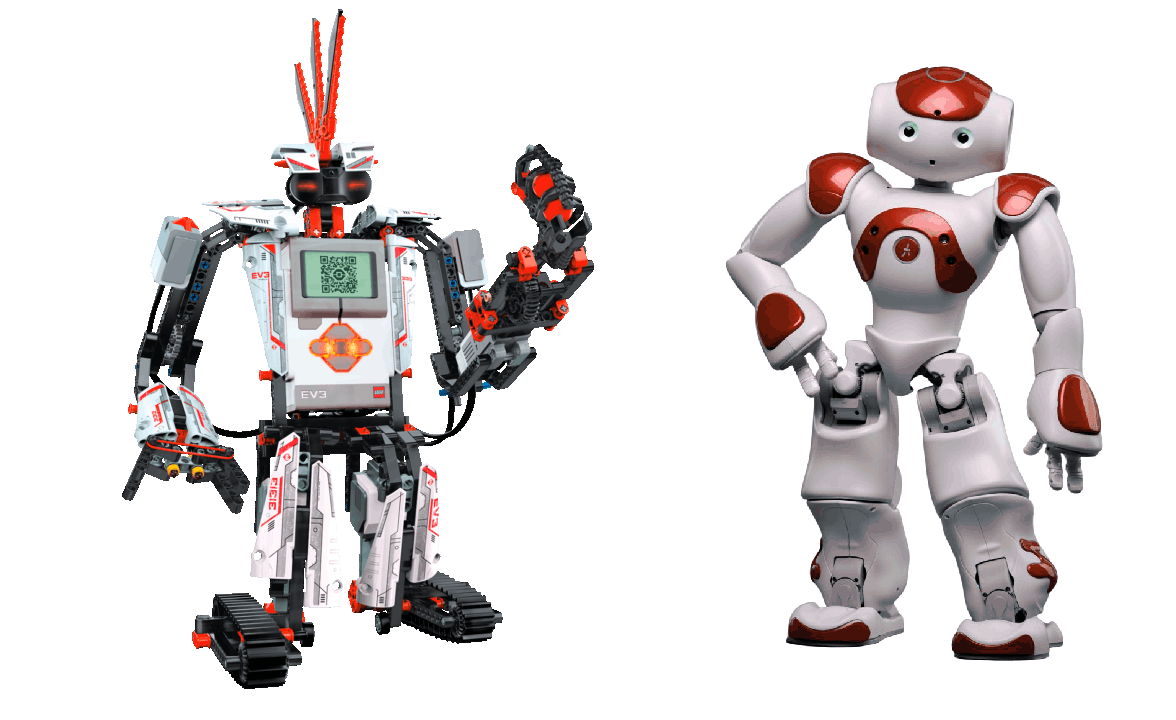
\includegraphics[width=300pt]{illustrations/ev3_nao.png}\\
\caption{Both the EV3 Lego Mindstorms (left) and the Nao (right) run a distribution of the Linux Kernel. \cite{EV3, NAO}} 
\label{central thread}

\end{figure}

\noindent
Considering all of the points previously mentioned Linux was picked as the target programming platform over any other alternatives. Linux's embeddable nature is important to this project as at least one of the physical robots may be equipped with the \textit{Raspberry Pi} a credit card size computer capable of running Linux. The system will be tested on two distributions of Linux, one embedded on the robot(s), the other connected externally:

\begin{itemize}
\item Raspbian (Embedded)
\item Ubuntu Linux 14.10 (External)
\end{itemize} 

\newpage

\subsection{Python3}
Python version 3 (Python3) has been selected as the most appropriate core programming language for the implementation stage for the following reasons:

\begin{itemize}
\item Development Speed - Python is an interpreted bytecode language which is compiled ``on the fly" eliminating lengthy build overheads.
\item Interactive Shell - Python's shell facilitates interactive programming which lends itself to test driven coding.
\item Python and Robotics - already widely used in the robotics field, Sebastian Thurn's Udacity program is done purely using Python \cite{THRUN}.
\end{itemize} 

\noindent
Python's syntax is also extremely lenient when compared to compiled languages such as C where every variable must explicitly declares its type before it can be used, making the equivalent Python code more visually compact. The implementation could have been carried out using C, C++, Java, or C$\sharp$ as the author already has the experience in those languages, however using Python instead presents a unique learning opportunity. 

\subsection{Cython Modules}
\noindent
A major drawback of interpreted languages is the speed of their execution when compared to compiled languages, since Python is implemented using a virtual machine it will nearly always be slower than pure machine code. It is important to take this issue into account at design time as the planning algorithms are computationally complex and as the state space increases Python will become less adapt at handling it compared to a compiled language. \\

\noindent
Fortunately as Python is wrote in C it can also be extend using C. Implementing the planning algorithms as Cython modules shall significantly increase their performance while still enabling the rest of the system to use Python. At the time of writing GCC (GNU C Compiler) version 4.9.1 has been selected for compilation purposes.

%-------------------------------------------------------------------------------------------------------

\newpage

\section{Source Control}
This section covers how the project was managed, the source control system used, frequency off commits, total commits, and any branching.

\subsection{Git}
\noindent
Throughout the projects development all work undertaken including everything from the code base, poster, modelling, and thesis was managed and controlled using the Git source control tool. This decision was taken at design time as it came with a number of distinct advantages such as providing a clear work history and the ability to roll back changes if the need arose. Another important reason for choosing Git over other systems is that it maintains a local copy in addition to the working head in the remote repository \cite{GIT}. An open repository was set-up and maintained in the cloud at the GitHub \href{https://www.github.com/swordmaster2k/botnav}{BotNav}.

\newpage

%-------------------------------------------------------------------------------------------------------

\chapter{Core Implementation}

%-------------------------------------------------------------------------------------------------------

\section{Building the Project}

\subsection{Obtaining the Source}
\noindent 
The latest version of the project's source code can be checked out via \textit{git} using: \\

\indent \textit{git clone https://github.com/swordmaster2k/botnav.git} \\

\noindent
Or downloaded as a ZIP file from \url{https://github.com/swordmaster2k/botnav}. \\ 

\noindent
Alternatively the most up to date version at the time of printing is available on the CD at the front of this thesis.

\subsection{Compiling the D* Lite Cython Module}
\noindent
The planning algorithm D* Lite must be compiled as a Cython module, the original source code was provided by Maxim Likhachev of CMU and Sven Koenig of USC in C. It has been modified to make it compatible with the core Python system using Cython, as Python is implemented in C \cite{•} it is inherently compatible with the sample of D* Lite that is provided by its authors.

\noindent
To build D* Lite you will need Python3.4, the Python3.4 headers, gcc, and make. It \textbf{must} be built for each platform on which it will execute as C compiles to machine code making it \textit{target dependent}. From a terminal navigate to the source code directory \textit{BotNav/algorithm/dstarlite\_build/}. \\

\noindent
The make file contains two build rules:
\begin{enumerate}
\item \textit{make} - \indent which builds the module \textit{dstarlite\_c.so} 
\item \textit{make clean} - \indent cleans all previous output files from the build process \\
\end{enumerate}

\noindent
Once the module file \textit{dstarlite\_c.so} has been successfully built for the target platform it can simply be dropped into the parent directory \textit{BotNav/algorithm/}. The Python source code contains a reference to the module and will automatically link it in at execution time. 

\subsection{Running it in Python3}
\noindent
By default the project is set-up to run a sample simulation with \textit{sample.map} using the GridNav path planning algorithm. It will output the results of its run to the \textit{BotNav/maps/output/} directory and is configured to compute a path from every traversable cell to the goal. To run it simply navigate to the path containing \textit{tester.py} and type: \\

\indent \textit{python3 tester.py config.botnav} \\

\noindent
The argument passed to \textit{tester.py} is the path to the default configuration file, the contents of which will be discussed later in this chapter. After running the above command in a terminal the result shall look similar to Figure \ref{sample_output}.

\begin{figure}[htbp]

\center 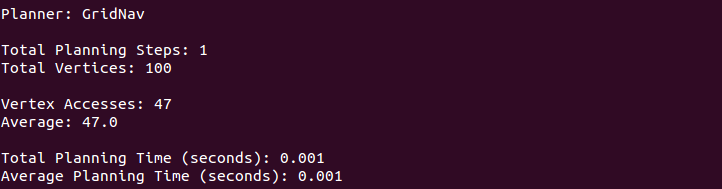
\includegraphics[width=435pt]{illustrations/sample_output}\\
\caption{An example of the type of output generated after running GridNav over \textit{sample.map} in simulation mode.} 
\label{sample_output}

\end{figure}

%-------------------------------------------------------------------------------------------------------

\section{Running Simulations}
\noindent
Simulations provide an easy means of testing each planning algorithm in controllable environments, it speeds up the testing process immeasurably, and provides reproduce-able results. The most powerful feature of simulations is the ability to plan a path from every free cell in the environment, the result of each traversal is placed into a separate timestamped folder. This data can then be easily mined and analysed in order to gauge how each algorithm performed for a particular scenario.

\subsection{Configuration}
\noindent 
When carrying out simulated runs three parameters must be set in the corresponding configuration file they are \textit{map}, \textit{mode}, and \textit{planner}. Below is an example of the configuration required to run a simulated trial using D* Lite: \\

	\indent \textit{map=maps/simple.map \\}
	\indent \textit{planner=d\_star\_lite \\}
	\indent \textit{mode=simulated \\}

\noindent
The most important parameter setting here is \textit{mode} which is set to simulated. At run time this informs the \textit{Tester} class that we want to run an experimental simulation across all traversable cells and that we do not need a communications channel via \textit{Proxy}. In simulation mode all of the instructions are invoked on the ``dummy'' robot class \textit{SimulatedRobot}, the method \textit{go\_to(self, x, y)} simply takes the $x$ and $y$ coordinates, introduces some random drift, and assigns them: \\

\begin{lstlisting}
def go_to(self, x, y):
	# Introduce a little uncertainty.
    self.x = (x + random.uniform(-0.2, 0.2)) * self.cell_size  
    self.y = (y + random.uniform(-0.2, 0.2)) * self.cell_size
    
    self.trail.append([self.get_cell_x(), self.get_cell_y()])
    
    self.state = "Travelled"
\end{lstlisting}

\subsection{Sample Output}

\begin{figure}[htbp]

\center 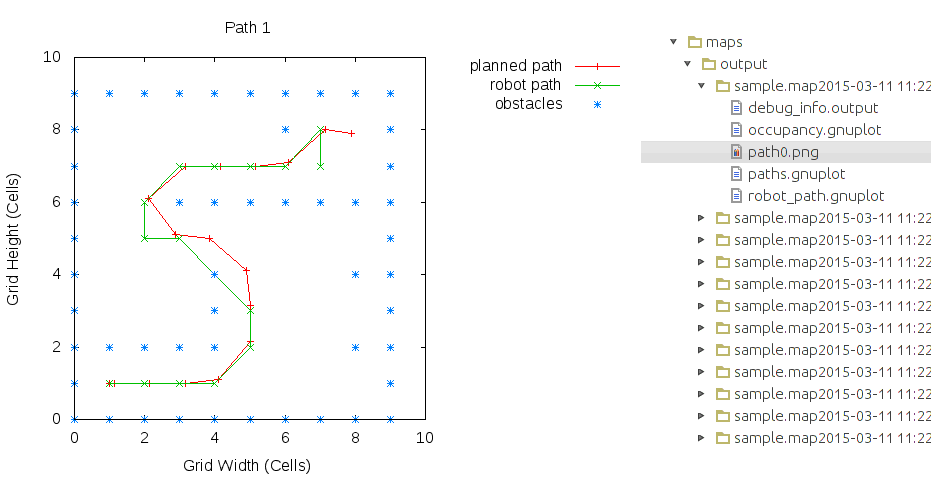
\includegraphics[width=435pt]{illustrations/sample_output_2}\\
\caption{A plot file for the first path from the sample map generated by \textit{gnuplot} (left), and the contents of the output folder after the run. Note that each folder is timestamped (right).} 
\label{sample_output}

\end{figure}

\newpage

%-------------------------------------------------------------------------------------------------------

\section{Using a Real Bot}
\noindent
The real test for any path planning algorithm is its practical effectiveness \cite{FIELD} and the only way to gauge this is using a physical robotic platform i.e.``a Real Bot''. The simulations that we have performed here are very limited in nature as they do not take into account any variability in the mechanics of the robot. While it is perfectly possible to model variations such as drift, odometry error, friction, and battery drain in a simulation it is far more practical to simply use a physical platform.  \\
  
\noindent
There are a number of factors that we must consider when using a physical robot, to begin with we will need some form of communications mechanism be it wired (USB, Ethernet, Serial) or wireless (ZigBee, WiFi, Bluetooth). It is through this medium that the \textit{Proxy} class will process the data to and from the robot. Then there is drift, occurrences such as wheel slippage can lead to the robot veering off course, we will assume that this issue is dealt with at a lower level than the path planning system.

\subsection{Configuration}
\noindent
The contents of the configuration file for a hardware robot depends on the communications medium being employed. At present the system supports three forms of communication Bluetooth, IP, and Serial. Before any of these can be used the run mode must set to \textit{physical}. Below is an example configuration using Bluetooth which requires the MAC address of the device and a port number: \\

	\indent \textit{map=maps/sample.map\\}
	\indent \textit{planner=grid\_nav\\}
	\indent \textit{mode=physical\\}
	\indent \textit{connection=bluetooth\\}
	\indent \textit{mac=00:00:12:06:56:83\\}
	\indent \textit{port=0x1001}
	
\noindent 
For IP based configurations an \textit{ip}, \textit{mac}, and \textit{port} setting will be required. Serial based connections need only a \textit{baud}, and \textit{port}, examples of both are available in the comments of the default configuration file: \\

	\indent \#   	\textit{if connection == bluetooth\\}
	\indent \#		\indent \textit{mac=\\}
	\indent \#      \indent \textit{port=\\}
	\indent \#   	\textit{elif connection == ip\\}
	\indent \#      \indent \textit{ip=\\}
	\indent \#      \indent \textit{mac=\\}
	\indent \#      \indent \textit{port=\\}
	\indent \#   	\textit{elif connection == serial\\}
	\indent \#      \indent \textit{baud=\\}
	\indent \#      \indent \textit{port=}

%-------------------------------------------------------------------------------------------------------

\section{How the Planner Works}
\noindent
As we have already seen our \textit{Planner} is implemented on its own separate thread which is designed to handle the bulk of the processing required to get our mobile robot from point a to b. All of this work is carried out within the \textit{run} method which is invoked when the thread is started. Below is a snippet of the code from the start of this method: \\

\begin{lstlisting}
'''
Step 1: Plan.
'''
self.algorithm.plan()

# Write the state after first planning step.
self.write_state()

# Append a copy of the path to our paths record.
paths.append(self.algorithm.path[:])

# Stick the starting position of the robot into
# the first path.
paths[0].insert(0, [self.robot.get_cell_x(), self.robot.get_cell_y()])

# Calculate our initial distance from the goal.
[output omitted]

# Write some debugging info.
self.write_debug_info()
\end{lstlisting}

\noindent
During the planning process the \textit{Planner} goes through a number of steps, part of the first step is outlined in the above code snippet. After the initial planning step that is used to evaluate if a path to the goal exists the planner immediately writes the state to our output files. Then some additions to the path collection are made including the robot's start position, the goal distance is calculated and checked, and lastly debugging information is recorded. This is just the first of five steps involved during the planning process this particular step only runs once per test. In the next section we will discuss all five steps together in \ref{steps}.

\subsection{Five Simple Steps}\label{steps}
\noindent
The planning process presented in this work was inspired by \cite{GRIDNAV95}. In \cite{GRIDNAV95} T. Balch established a simple methodology that enabled a mobile robot equipped with grid based planner to successfully navigate towards its goal in an iterative manner using seven steps. Those steps can be seen on page 7 of his paper. Our planning process was originally derived from these steps and later simplified by reducing it from seven steps to five:

\newpage

\begin{enumerate}
\item Plan.
\item Scan the immediate area for obstacles and free space.
\item Update the map if necessary.
\begin{enumerate}
\item Recompute the plan if necessary.
\end{enumerate}
\item Pop the next point from the current path and travel.
\item Go to 2.
\end{enumerate}

\noindent
In the original version the initialisation of variables and the reading of the map file were included as a step, this is not included in the \textit{Planner} directly so it was removed. Also step 5 from \cite{GRIDNAV95} became the optional step 3(a) as this step will only ever be taken if the condition for step 3 becomes \textit{true}. This process will iteratively execute from step 2 through 5 until either the goal is reached \textit{or} when no path can be found. Essentially all of the work in this entire project evolved from this methodology. By reading over \cite{GRIDNAV95} we can gain a fundamental understanding of everything that grid based path planning involves from start to finish. 

\subsection{Abstracting Away from the Algorithm}
\noindent
Art the heart of the object oriented patterns used in this project is \textit{abstraction}, a technique that enables a developer to generalise the functionality of a class through abstract inheritance. Through this process the complexity of an object can be reduced and its efficiency greatly increased \cite{http://whatis.techtarget.com/definition/abstraction}. It has been used extensively in the implementation of the path planning algorithms which all inherit from the base class \textit{AbstractAlgorithm}. From this class each algorithm inherits a series of default behaviours some of which are listed here:

\newpage

\begin{itemize}
\item plan(self) -
\item pop\_next\_point(self) - 
\item print\_debug(self, stream) - 
\end{itemize}

\noindent
The real advantage to using abstraction here is the \textit{pluggable} nature it provides. Every algorithm that inherits from the \textit{AbstractAlgorithm} base class implements a common set of behaviours and properties. Regardless of which algorithm is currently being used for planning we simply access the same behaviour or property (see Figure \ref{abstraction_method}). The implementation details of each algorithm is hidden from the \textit{Planner} whom only cares about the results.

\begin{figure}[htbp]

\center 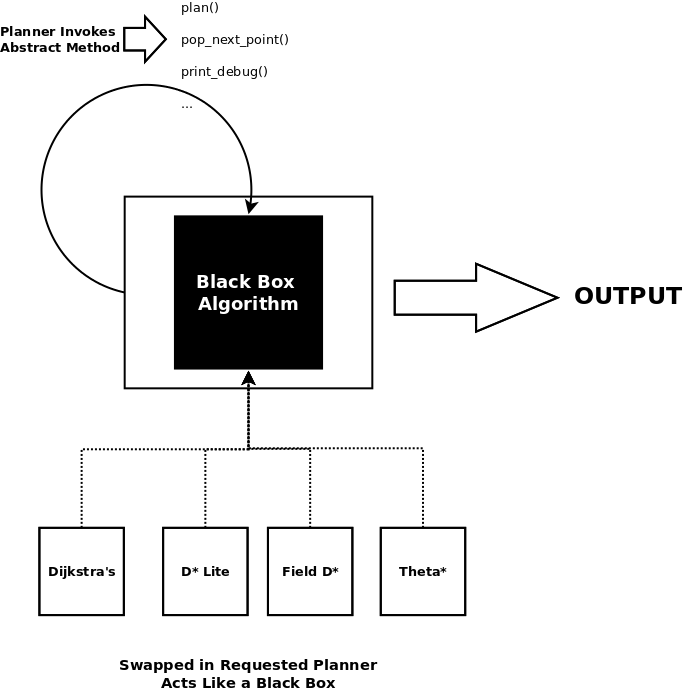
\includegraphics[width=290pt]{illustrations/abstraction}\\
\caption{The current algorithm acts as a black box to the \textit{Planner} whom calls a set of public abstract methods. Any planning algorithm can be swapped in for testing without having to account for its implementation specifics.} 
\label{abstraction_method}

\end{figure}

%-------------------------------------------------------------------------------------------------------

\newpage

\section{Open Field D*}
\noindent
For implementation purposes we modified sample implementations of Dijkstra's Algorithm, D* Lite, Theta*, and then plugged them into the path planning system. This made perfect sense as we saw no point in reinventing the wheel and coding all of these algorithms from scratch. However there was one algorithm for which no \textit{public} implementation existed. Field D* has provided advance path planning capabilities to some of the most sophisticated robots ever made including NASA's Curiosity rover and the GDRS XUV \cite{FIELD}. Its authors claim that Field D* is an efficient planning and replanning algorithm that can produce smooth paths costing on average 4\% less than traditional planners \cite{FIELD}. \\

\noindent
Verifying the claim made by the authors of Field D* requires a working implementation, the problem is that all existing work on Field D* has been carried out behind closed doors mostly at NASA. To the best of our knowledge the work presented here contains the first openly available version of Field D* nicknamed appropriately \textit{Open Field D*}. In order to derive our version of this novel path planner we based it on the basic D* Lite version presented on the $8^{th}$ page of \cite{FIELD} which can be seen below:

\begin{figure}[htbp]

\center 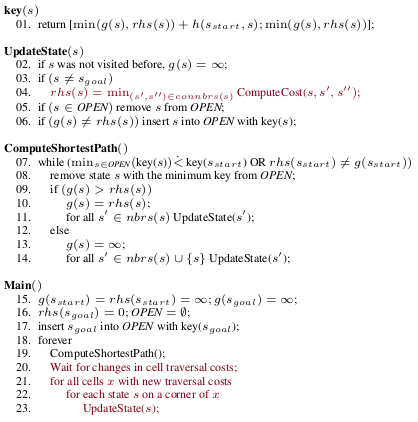
\includegraphics[width=200pt]{illustrations/field_d_basic}\\
\caption{} 
\label{field_d_basic}

\end{figure}

\subsection{Basic Implementation}

\noindent
The basic version of Field D* differs little from the original specification of D* Lite except when it comes to updates. In the literature review we mentioned how Field D* shifts nodes from cell centres to cell edges which can be seen in Figure \ref{Figure: Optimal.}. Equipped with this modification Field D* can produce smooth paths using linear interpolation techniques that enable a path to intersect any point on the edge of a cell. Calculating the cost of a node requires all its consecutive neighbours (node pairs) that represent the neighbouring edges. This operation can be seen on line 4 in Figure \ref{field_d_basic}. After a detailed analysis of the \textit{pseudo code} we came up with the following solution in Python: \\

\begin{lstlisting}
def get_consecutive_neighbours(self, s):
        consecutive_neighbours = []

        for i in range(len(self.NEIGHBOUR_DIRECTIONS)):
            try:
                if i == len(self.NEIGHBOUR_DIRECTIONS) - 1:  # Edge s8 -> s1
                    x1 = s.x + self.NEIGHBOUR_DIRECTIONS[i][0]
                    y1 = s.y + self.NEIGHBOUR_DIRECTIONS[i][1]
                    x2 = s.x + self.NEIGHBOUR_DIRECTIONS[0][0]
                    y2 = s.y + self.NEIGHBOUR_DIRECTIONS[0][1]

                    if x1 > -1 and y1 > -1 and x2 > -1 and y2 > -1:
                        consecutive_neighbours.append(
                            (self.nodes[s.x + self.NEIGHBOUR_DIRECTIONS[i][0]][s.y + self.NEIGHBOUR_DIRECTIONS[i][1]],
                             self.nodes[s.x + self.NEIGHBOUR_DIRECTIONS[0][0]][s.y + self.NEIGHBOUR_DIRECTIONS[0][1]]))
                else:  # All other edges.
                    x1 = s.x + self.NEIGHBOUR_DIRECTIONS[i][0]
                    y1 = s.y + self.NEIGHBOUR_DIRECTIONS[i][1]
                    x2 = s.x + self.NEIGHBOUR_DIRECTIONS[i + 1][0]
                    y2 = s.y + self.NEIGHBOUR_DIRECTIONS[i + 1][1]

                    if x1 > -1 and y1 > -1 and x2 > -1 and y2 > -1:
                        consecutive_neighbours.append(
                            (self.nodes[s.x + self.NEIGHBOUR_DIRECTIONS[i][0]][s.y + self.NEIGHBOUR_DIRECTIONS[i][1]],
                             self.nodes[s.x + self.NEIGHBOUR_DIRECTIONS[i + 1][0]][
                                 s.y + self.NEIGHBOUR_DIRECTIONS[i + 1][1]]))

            except IndexError:
                pass
            except AttributeError:
                pass

        return consecutive_neighbours
\end{lstlisting}

\noindent
Essentially what we are doing in the above code sample is iteratively processing all the neighbouring node pairs in a clockwise direction to get the sequence $\lbrace \overrightarrow{s_{1}s_{2}}, \overrightarrow{s_{2}s_{3}}, \overrightarrow{s_{3}s_{4}}, \overrightarrow{s_{4}s_{5}}, \overrightarrow{s_{5}s_{6}},$ $\overrightarrow{s_{6}s_{7}}, \overrightarrow{s_{7}s_{8}}, \overrightarrow{s_{8}s_{1}} \rbrace$. We can then compute the cost of node \textit{s} by selecting the lowest costing neighbour pair and calling the following function: \\

\begin{lstlisting}
def compute_cost(self, s, sa, sb):
        self.vertex_accesses += 1
        s.evaluations += 1

        [output omitted]

        # Map mid_x and mid_y to a cell cost, if the x and y is out of
        # bounds c == LARGE.
        c = self.get_cell_cost(math.floor(mid_x), math.floor(mid_y))

		[output omitted]

        if min(c, b) == self.BIG_COST:
            vs = self.BIG_COST
        elif s1.g <= s2.g:
            vs = min(c, b) + s1.g
        else:
            f = s1.g - s2.g

            if f <= b:
                if c <= f:
                    vs = c * SQRT_2 + s2.g
                else:
                    y = min(f / (math.sqrt(c ** 2 - f ** 2)), 1)
                    vs = c * math.sqrt(1 + y ** 2) + f * (1 - y) + s2.g
            else:
                if c <= b:
                    vs = c * SQRT_2 + s2.g
                else:
                    x = 1 - min(b / (math.sqrt(c ** 2 - b ** 2)), 1)
                    vs = c * math.sqrt(1 + ((1 - x) ** 2)) + (b * x) + s2.g

        if vs > self.BIG_COST:
            vs = self.BIG_COST

        return round(vs, 3)
\end{lstlisting}

\noindent
Cost calculation in Field D* is based on \textit{g-values} and also the estimated traversal cost of the selected neighbouring cell which can vary. The above Python code is a direct implementation of the mathematical theory presented on page 7 of \cite{FIELD}. It is not possible to cover the algorithm in-depth here due to its length, further reference should be should be sought from \cite{FIELD, FIELD2} and this project's source code.

\subsection{Issues with Field D*}
\noindent
The most challenging part of this project was by far the implementation of Field D*. Little information on the algorithm exists beyond what is included in \cite{FIELD, FIELD2} despite the fact that it dates back to 2007 \cite{FIELD}. Thankfully Field D* was originally derived from D* Lite \cite{D*LITE} and its basic version simply extend its. With that said we encountered a large number of ambiguities that required us to mathematically reverse engineer some of its specification. One aspect that remains unclear is path extraction which is not covered in any level of detail by the authors. \\

\noindent
Every node in the Field D* cost grid can be seen as a sample point in a continuous space, when extracting a path we select the lowest costing edge. The cost of an edge is the sum of both connecting nodes, our optimal path intersects this edge at some point $(x, y)$. Exactly how this point is obtained is never clearly defined. In our implementation we extract our new point based on the \textit{rhs-values} of the nodes $s_{1}$ and $s_{2}$, which we then shift based on the direction of travel: \\

\begin{lstlisting}
f = s1.rhs - s2.rhs

if f > 1:
	f = 1
elif f < -1:
	f = -1

x_difference = s1.x - s2.x
y_difference = s1.y - s2.y
x_shift = 0
y_shift = 0

if x_difference != 0:
	if x_difference < 0:
		x_shift = f
	else:
		x_shift = -f
else:
	if y_difference < 0:
		y_shift = f
	else:
		y_shift = -f

if x_shift != 0:
	self.s_start.x += x_shift
	self.s_start.y = s2.y
elif y_shift != 0:
	self.s_start.x = s2.x
\end{lstlisting}

\noindent
This method works well for most of the cases that we tested it against, however it breaks down in complex environments that are obstacle dense. While we have not been able to solve this part of Field D*, the rest of the algorithm functions as expected. It is possible to produce smooth and low costing paths using our implementation for 80\% of the cases that we tried. Hopefully overtime the work can be improved and a fully functioning version of Field D* will exist outside of NASA.

\newpage

\section{Hardware Platform}
\noindent
We will now take the time to briefly discuss the specification of the physical robot that was used through the course of this project. All of the hardware was sourced from suppliers outside of Ireland, mostly from China and the UK. The robotic platform was built upon the DFRobot Cherokey 4WD that comes with an integrated motor driver and communications circuity. The robot's computing power is based on a mounted Arduino Mega 2560, a Bluetooth link is provided by the JY-MCU module, and MPU6050 gyroscope combined with wheel encoders is used for positioning. The robot was completely custom built to meet the needs of the planning system. \\

\noindent
There are a number of pre-built robotic kits that can provide this functionality of the shelf but they are typically more expensive than building. Also by constructing the robot from the ground up we maximised our level of learning as we covered robotics from both a software and engineering perspective. However the robot is essentially ``dumb'' and blind to the world around it knowing only its position, the bulk of the processing is done on the other side of the communications link. Our platform implemented the interface that we specified in \ref{hardware_specification}.

\newpage

\subsection{Odometry Gathering}
\noindent
The position of the robot in its 2D environment is established using both the linear distance provided by the encoders and the current heading from the gyroscope. The wheel encoders give us the tick count for each wheel, we can come up with a distance based on the number of ticks a wheel goes through during a complete rotation. For our robot there is a total of twenty ticks each accounting for a distance of $0.010205m$. Given the distance travelled we can determine our change in position using the \textit{cos} and \textit{sin} of our current heading: \\

\begin{lstlisting}
if (deltaDistance != 0.0)
{
	if (state == GOING_BACKWARD)
	{
		deltaX = (deltaDistance) * cos(-theta);
		deltaY = (deltaDistance) * sin(-theta);
	}
	else
	{
		deltaX = (deltaDistance) * cos(theta);
		deltaY = (deltaDistance) * sin(theta);
	}

	x += deltaX;
	y += deltaY;
}
\end{lstlisting}

\newpage

\subsection{Issues}
\noindent
Our hardware implementation was not without issues and during the course of its development we faced numerous challenges, perhaps the most serious one being \textit{drift}. The Cherokey's drive system is based on a set of four small geared DC motors, its wheels are attached directly to the drive shaft without any extra fixings. During travel there is a tendency for these wheels to slip, particularly during rotations. This slippage is then registered as false ticks which throws our odometry off. In an attempt to counter the drift we calculated its average effect over a carpeted surface: \\

\begin{lstlisting}
const double DISTANCE_PER_TICK = 0.010205;

deltaX += X_DRIFT_CARPET * (deltaX / 0.01);
deltaY += Y_DRIFT_CARPET * (deltaY / 0.01);
\end{lstlisting}

\noindent
During rotations slippage was so bad that we were forced to use pure rotations, meaning we assume that the robot's position does not change while rotating. Another issue that progressively affects the robot is rotational drift, the MPU6050 gyroscope's heading changes by $0.01rad$ every couple of minutes. It is not a problem for our application as the robot is used for short bursts, but it is worth taking note of. \\

\noindent
Lastly as with all things electronic there is the question of battery life, our robot was powered by a 8.4v 1600mAH airsoft gun battery pack. This gave between 5-10 minutes of usable performance after that the power levels were too low to support all the electronics at the same time. When the battery level reached its low point the robot would go into random spins or simply drive aimlessly forward. This made extensive hardware based tests completely impractical, it also highlighted the fact that a robot is only as useful as its battery's charge.

%-------------------------------------------------------------------------------------------------------
%\chapter{Testing}

%----------------------------------------------------------------------------------------------------------------------

\section{Test Cases}

\noindent
In this section we will establish our testing methodology that shall be used to answer our main research question. The purpose of these tests is to discover what is more important in path planning for mobile robots, computation speed, or shorter path lengths. To achieve this we have defined two test cases that look at: 

\begin{itemize}
\item Traversal time based on the path length.
\item Estimated computation time for vertex accesses.
\end{itemize}

\noindent
Examining what proportion the computation time takes when compared to the travel time will help us answer our main research question. The most efficient planner will be selected based on the combined traversal and computation time. Before we carry out these tests we must be aware of potential biased scenarios, for example in a maze like environment where movement is completely restricted to headings of $\dfrac{\pi}{4}$ all planners shall have similar performances. Another case is where our path travels through wide open spaces containing large numbers of free cells. Planners that focus their search using \textit{heuristics} \cite{feurg paper} have a distinct advantage here (D* Lite, Field D*, Theta*). 

\newpage

\subsection{Test Case 1: Path Length}\label{test 1}

\noindent 
Each of the planners produce one key output and that is a path from our start position to the goal. A property that all of these paths share in common is their physical length in metres. The goal of all of these planners is to compute the shortest path from the robot's current position to the goal. In order to determine on average which of the planners produces the best result for a given scenario we will examine the time it takes to traverse. \\

\noindent
Based on a large number of evaluations from every possible starting position to the goal for a given map it will be possible to say which planning algorithm on average produces the shortest path. To make this test fair it shall be based on a theoretical mobile robot with the following properties: 

\begin{itemize}
\item Average Speed: $0.6m/s$
\item Turning Speed: $1rad/s$ 
\end{itemize} 

\noindent
These figures were gathered from the performance of the DFRobot Cherokey 4WD platform during path traversals. It is important to note here that we are assigning a time penalty for turning which requires deceleration. Calculating the cost using this theoretical model reduces the error rate in our results as we do not have to deal with drift or other physical properties that affect real robot platforms. It also reduces the time it takes to test as we can now perform thousands of simulated runs at once. \\

\noindent
\textbf{Expected Result:} based on the claims of the authors of Field D* and Theta* we expect that the planners capable of dealing with headings other than $\dfrac{\pi}{4}$ will perform better.

\newpage

\subsubsection{Cost Calculation}

\noindent
The time it takes to traverse a path is then based on two inputs:

\begin{itemize}
\item Path length in metres.
\item Total heading change in radians.
\end{itemize}

\noindent
We can extract these two inputs from our raw path of points. The path length is simply the sum of all the distances between every point using the coordinate geometry distance formula: \\

\indent $d = \sqrt{(x_{2} - x_{1})^{2} + (y_{2} - y_{1})^{2}}$ \\

\noindent
Which can be implemented in \textit{psuedocode} as: \\

\begin{lstlisting}
length = 0

for each point in path:
	next_point = point.next()
	
	if next_point is not null:
		length += math.sqrt((next_point.x - point.x) ^ 2 + (next_point.x - point.x) ^ 2)
\end{lstlisting}

\noindent
The total number of headings changes is just the sum of the difference between our current heading at a point and the change in direction required to face the new point. Our equation for calculating the cost of traversing a path is then: \\

\indent $time = path\_length \times 0.6 + total\_rotations \times 1.0$ \\

\newpage

\subsubsection{Example}

\noindent
\textbf{Given:} path of $3m$ containing a total heading change of $1rad$. \\

\noindent
Based on the equation we just defined we can get the path cost by substitution: \\

\indent $\Rightarrow time = path\_length \times 0.6 + total\_rotations \times 1.0$ \\
\indent $\Rightarrow time = (3) \times 0.6 + (1) \times 1.0$ \\
\indent $\Rightarrow time = 5 + 1$ \\
\indent $\Rightarrow time = 6s$ \\

\noindent
We can use the result from this simple computation during our comparative analysis to determine which planner is producing the lowest costing path. The result can also help in calculating the resources required to reach the goal \textit{i.e.} battery drain, as time spent moving costs a significant amount of energy.

\subsection{Test Case 2: Vertex Accesses}\label{test 2}

\noindent
In order to properly address our main research question we must look at one other function that all the path planners perform during the planning process. When it comes to path planning algorithms the highest costing operation is anything that involves accessing a \textit{vertex}. Depending on the planners representation a vertex can either be a cell or an edge, vertices are accessed during cost calculation, updates, and traversals. It makes sense then to take into account the time spent accessing vertices while the path is being generated. \\

\noindent
While raw execution time may seem like a more obvious measure, the problem with it is that it depends on the underlying computer architecture. If we were to base our tests on the time the process spends in the processor they would be \textit{machine dependent} and difficult to reproduce \cite{FIELD2}. Instead we will adopt the same approach as in Test Case 1. \\

\noindent
Given the number of vertices accessed during the planning we can assign a constant time cost for every access independently of the processor. This works in practice as all of the planners use simple mathematical calculations when working with vertices. This allows us to safely establish a theoretical execution time. The value of this constant is not important as long as it is realistic and consistent across all tests:

\begin{itemize}
\item Cost per access: 100$\mu$s
\end{itemize}   

\noindent
\textbf{Expected:} it is expected the planners that focus their search will access less vertices and therefore use less computation time.

\subsubsection{Cost Calculation}

\noindent
Calculating the time cost for accessing vertices requires the following formula: \\

\indent $time = total\_accesses \times cost\_per\_access$

\subsubsection{Example}

\noindent
\textbf{Given:} the planner evaluated 400 of 2500 vertices for Test Case 1. \\

\indent $\Rightarrow time = total\_accesses \times cost\_per\_access$ \\
\indent $\Rightarrow time = (400) \times 100$ \\
\indent $\Rightarrow time = 0.04s$ \\

\noindent
The total time spent for both Test Case 1 and 2 is 6.04s, as a percentage the time spent planning is 1.51\%.  What we shall be looking to establish during the testing phase is which is more proportionally important fast planning or a shorter path.
%\chapter{Conclusion}

Wrap up the entire project with a 1 page conclusion that covers:

\begin{itemize}
\item The outcome of the project success or failure.
\item Significance of the findings.
\item Any big challenges that were overcome.
\item Outstanding issues or bugs that remain.
\item Anything that could have been done differently.
\item Learning outcome of the project.
\end{itemize}

%\chapter{Further Work}

%-------------------------------------------------------------------------------------------------------

It is hard to predict what any further work maybe at this stage but some possible suggestions will include:

\begin{itemize}
\item Modelling uncertainty in the robot's movements.
\item Developing an advanced graphical user interface.
\item Improving the robot's pose estimation using SLAM.
\item Accommodating more sensor models than just LIDAR.
\end{itemize}

\bibliography{bibliography}

%\appendix
\nonumchapter{Appendices}

\section{Communications Protocol Specification}\label{Appendix: Communications Protocol Specification} 
Full listing for the communications protocol used here explaining:


\begin{itemize}
\item Connection Types.
\item All possible Commands.
\item All possible Responses.
\item Example usage.
\end{itemize}

\newpage

\section{ITB DFRobot Pirate Platform}\label{Appendix: ITB DFRobot Pirate Platform}
Detailed explanation of the ITB's robot platform that was used with this project. Include all the pin configurations to sensors, circuit diagrams. Mention anything else of particular importance.

\newpage

\section{Source Code Listings}\label{Appendix: Source Code Listings}

\subsection{Planner}\label{Appendix: Planner}
Dump the full source code for the Planner class here when it is ready, include the whole thing.

\subsection{Field D* Algorithm}\label{Appendix: Field D* Algorithm}
Dump the most important parts of the Field D* Algorithm here when it is ready. Do not include all of it because it is likely to be 1000+ lines of code.

\section{Project Plan}
Modify the original project plan to suit the final outcome/work flow of the project and place it here once done.


\end{document}